% TODO reproducibility (sort out pickle), comments, PCA

% !TEX TS-program = xelatex
% !TEX encoding = UTF-8

\documentclass[a4paper, 11pt, twocolumn, final]{article} % use larger type; default would be 10pt

\usepackage{default}

\defaultfontfeatures{Mapping=tex-text}
\setmainfont[Ligatures=TeX]{Linux Libertine}

% \usepackage[parfill]{parskip} % Activate to begin paragraphs with an empty line rather than an indent

\usepackage{graphicx} % support the \includegraphics command and options
\usepackage{bm}

\title{Principal Component Analysis and Competitive Learning of MNIST Data}
\author{Joe MacMahon, University of Sheffield}
\date{\today}

\begin{document}
\maketitle

\begin{abstract}

This report details my study and application Principal Component Analysis and
Competitive Learning to the MNIST dataset of handwritten digits \cite{mnist}.
We\footnote{In reality, `we' is just me, but using it makes things a bit easier
to read.} used a Python-based approach with NumPy \cite{numpy} as a backend, and achieve an
error rate of 32\%.

In the report, we present a brief introduction to PCA and analyse the first five
principal components of the data, and then detail the neural network set-up and
algorithm used to build a classifier.

\end{abstract}

\section{PCA} A full introduction to PCA in any mathematical depth would be
outside the scope of this report, and can be found in any introductory machine
learning textbook.  However, we briefly state that PCA finds an ordering of
perpendicular axes (Principal Components) such that the projection of the data
onto the first principal component axis gives the largest spread of any
projection of the data, and each axis (a) is perpendicular to the rest and (b)
spreads the data wider than any subsequent axes.  Thus by composing a vector of
projections onto the ordered principal component axes, we obtain a vector whose
first component varies greatly with the data and each subsequent component
varies slightly less. For data of dimension $d$, this allows us to reduce its
dimensionality by considering the projection of the data onto the first $k$
principal component axes, for some $k < d$.  Through some mathematical
manipulation, it can be shown that the unit vectors of each principal component
axis are the eigenvectors of the covariance matrix of the data.

Using the Python library NumPy to calculate a covariance matrix and perform fast
matrix multiplication, we perform PCA on the MNIST dataset and take the first 5
principal components. Then we choose 3 of these 5 components and plot them to a
3-D graph.\footnote{This answers question 1 of part 1.  For details of the
algorithm and code snippets please see \autoref{sec:code}.} The results of this
can be seen in \autoref{fig:pca_graphs}.

\begin{figure}
  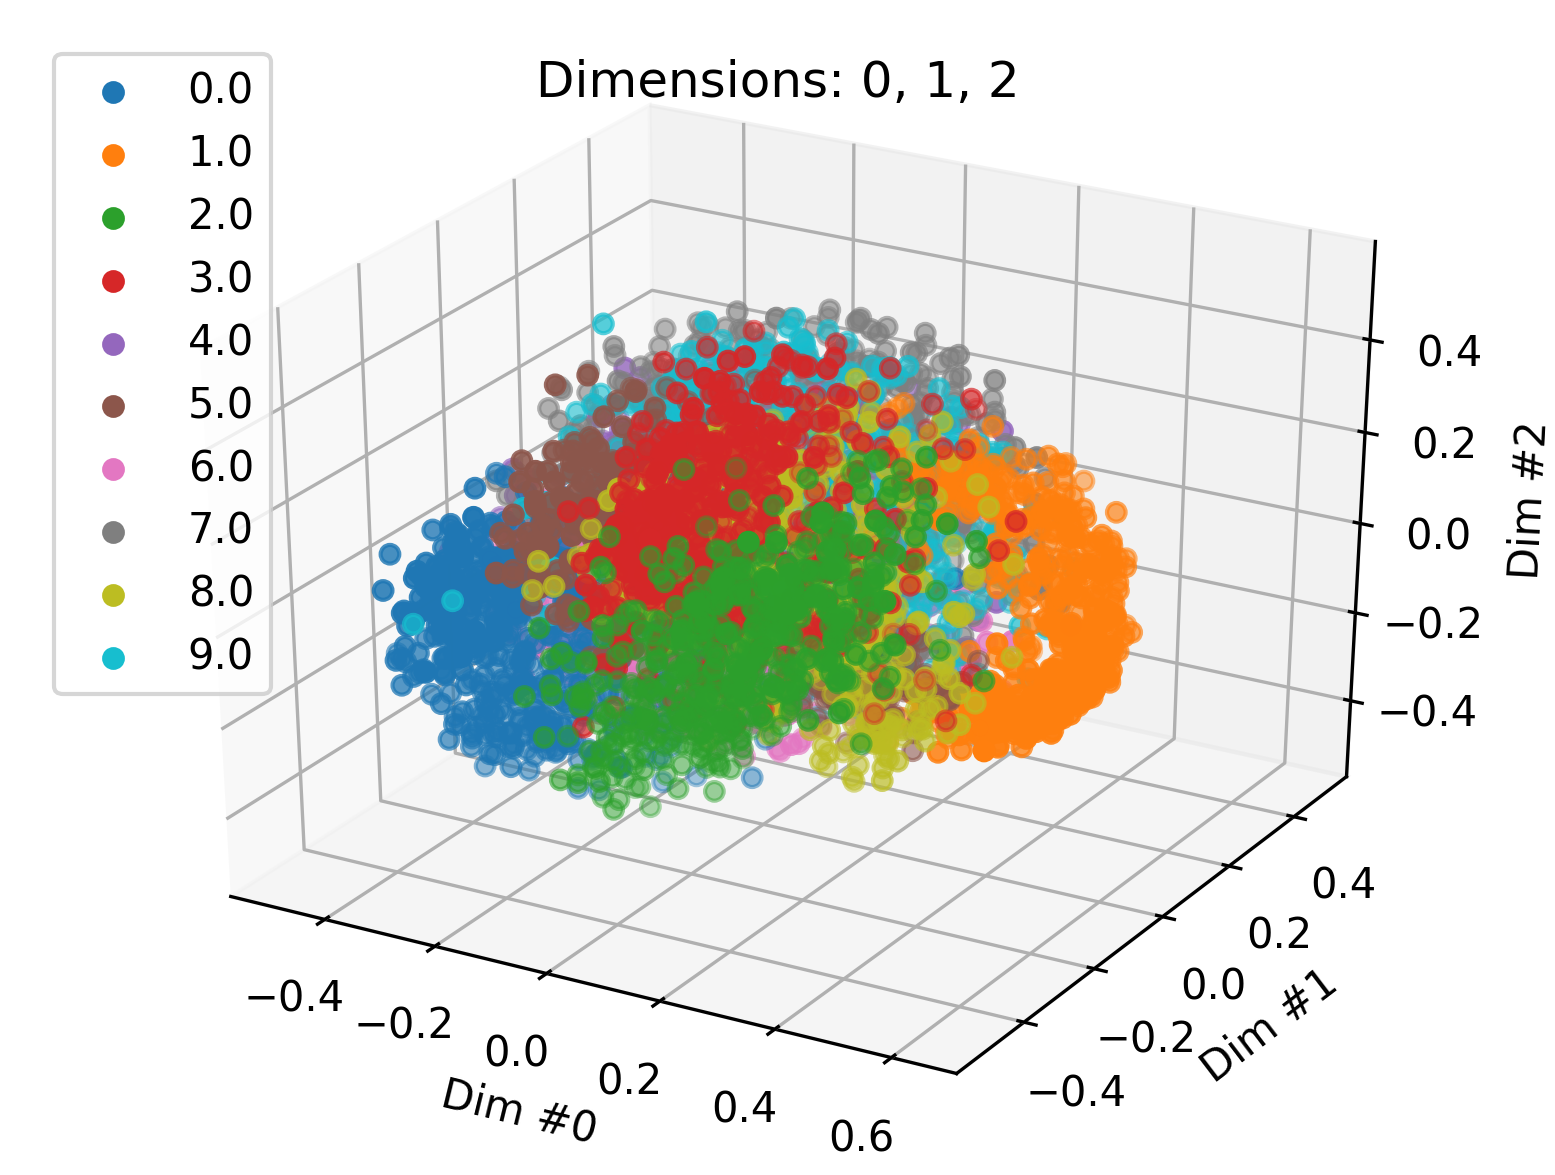
\includegraphics[width=0.23\textwidth]{pca/012.png}
  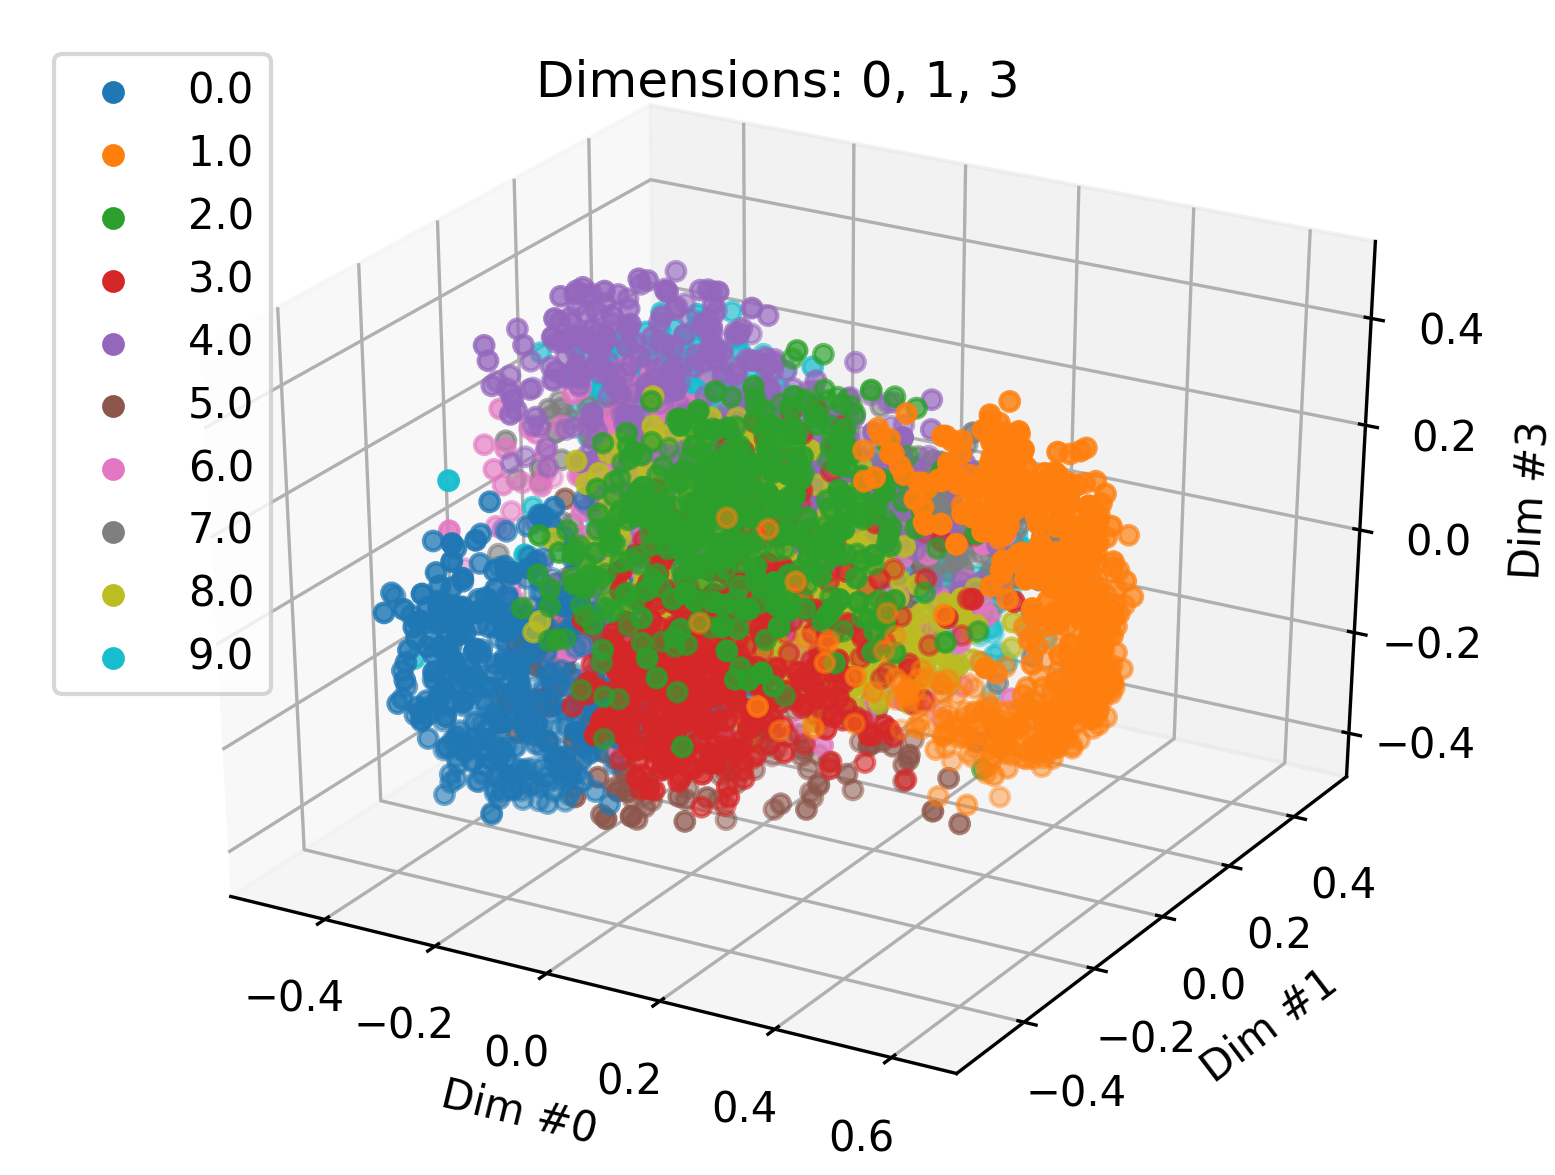
\includegraphics[width=0.23\textwidth]{pca/013.png}
  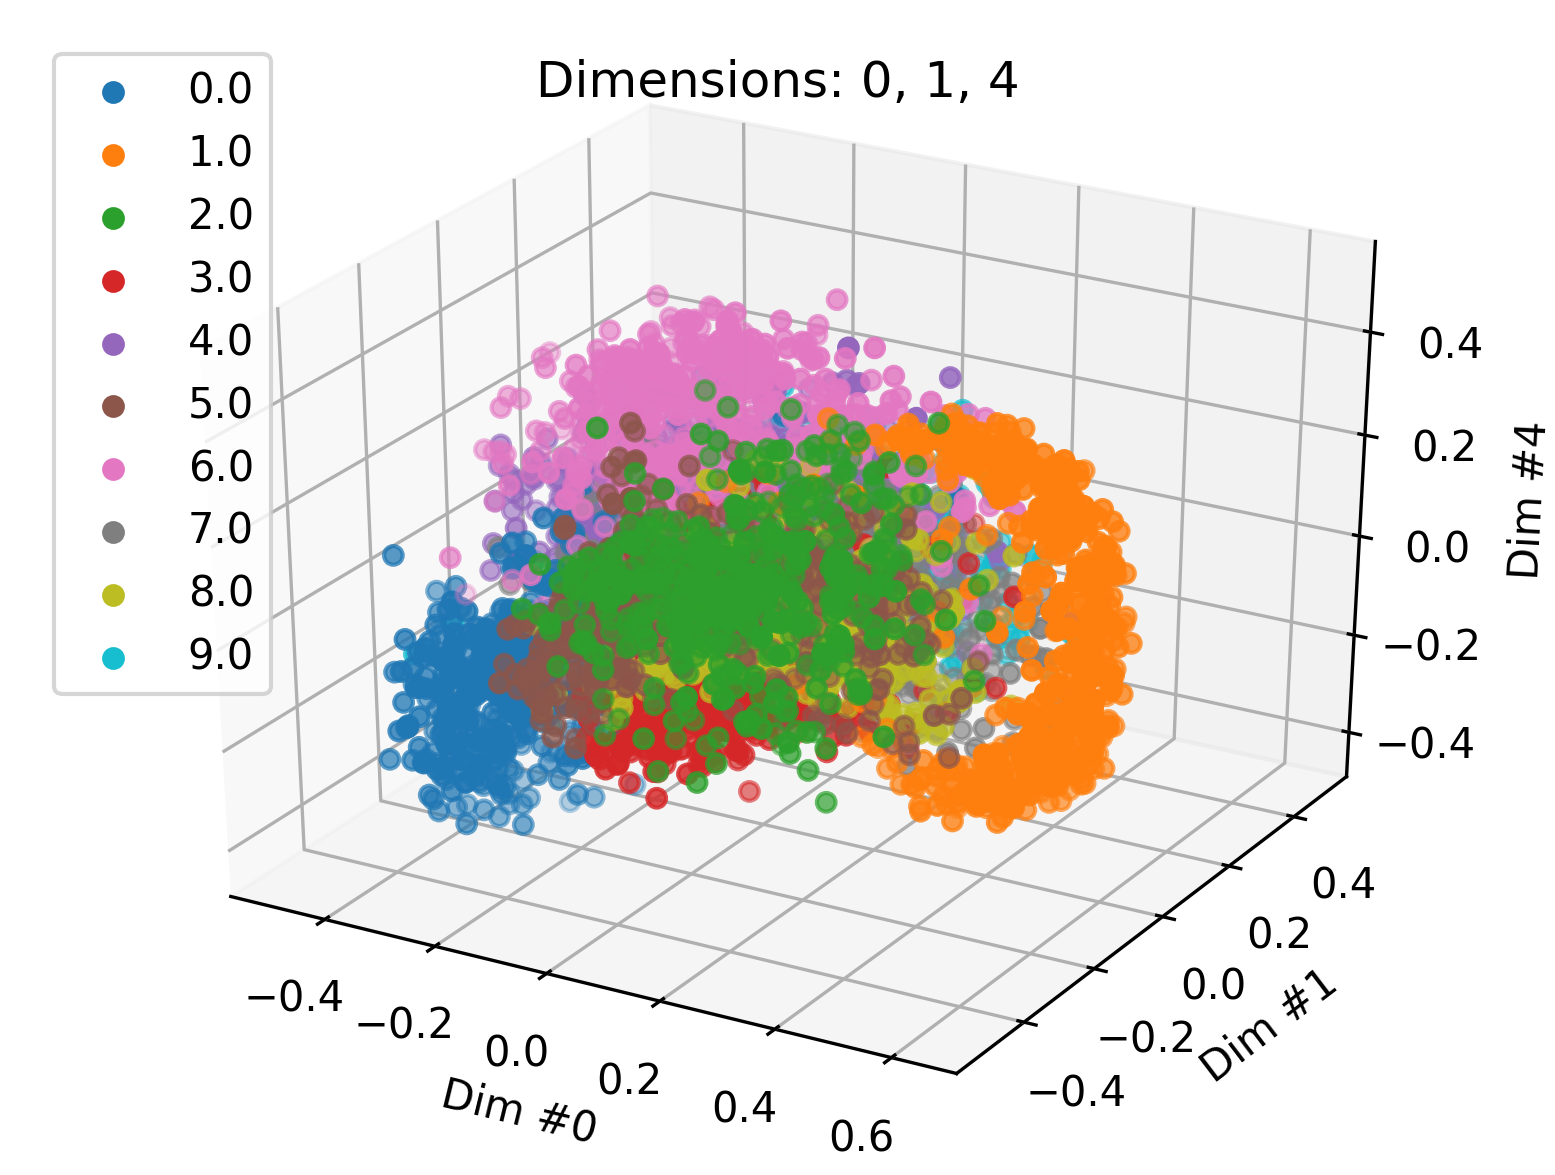
\includegraphics[width=0.23\textwidth]{pca/014.png}
  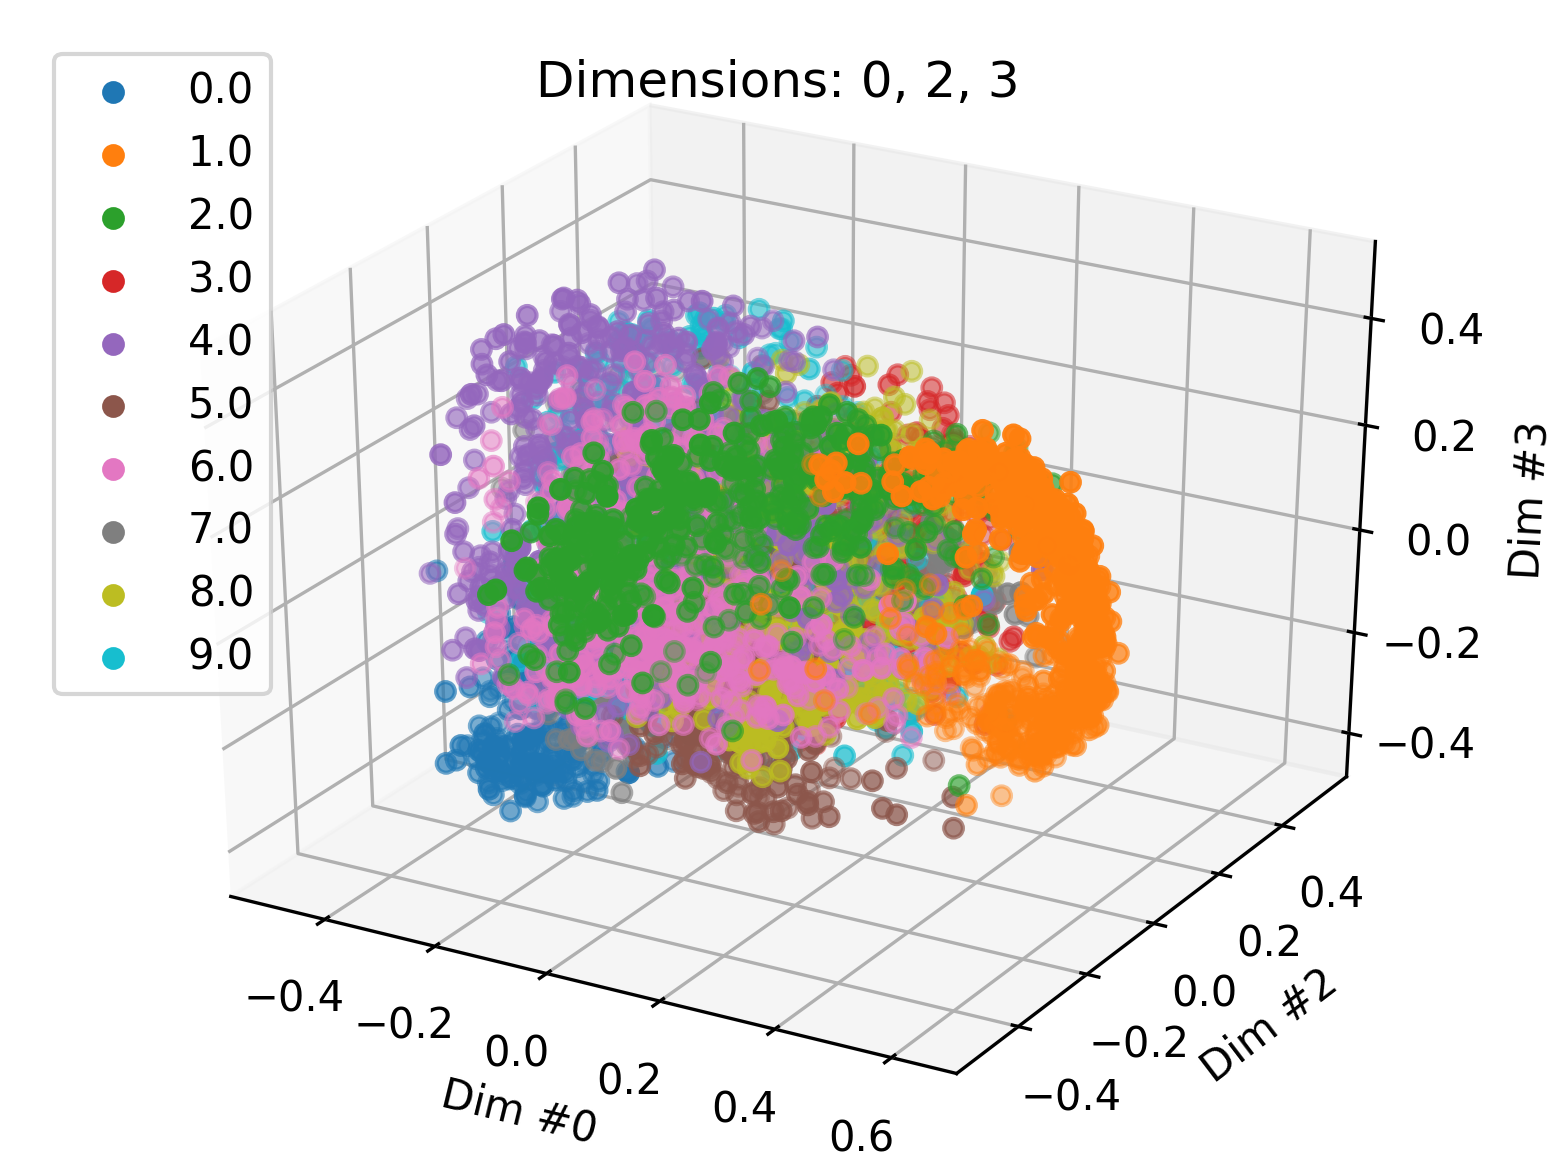
\includegraphics[width=0.23\textwidth]{pca/023.png}
  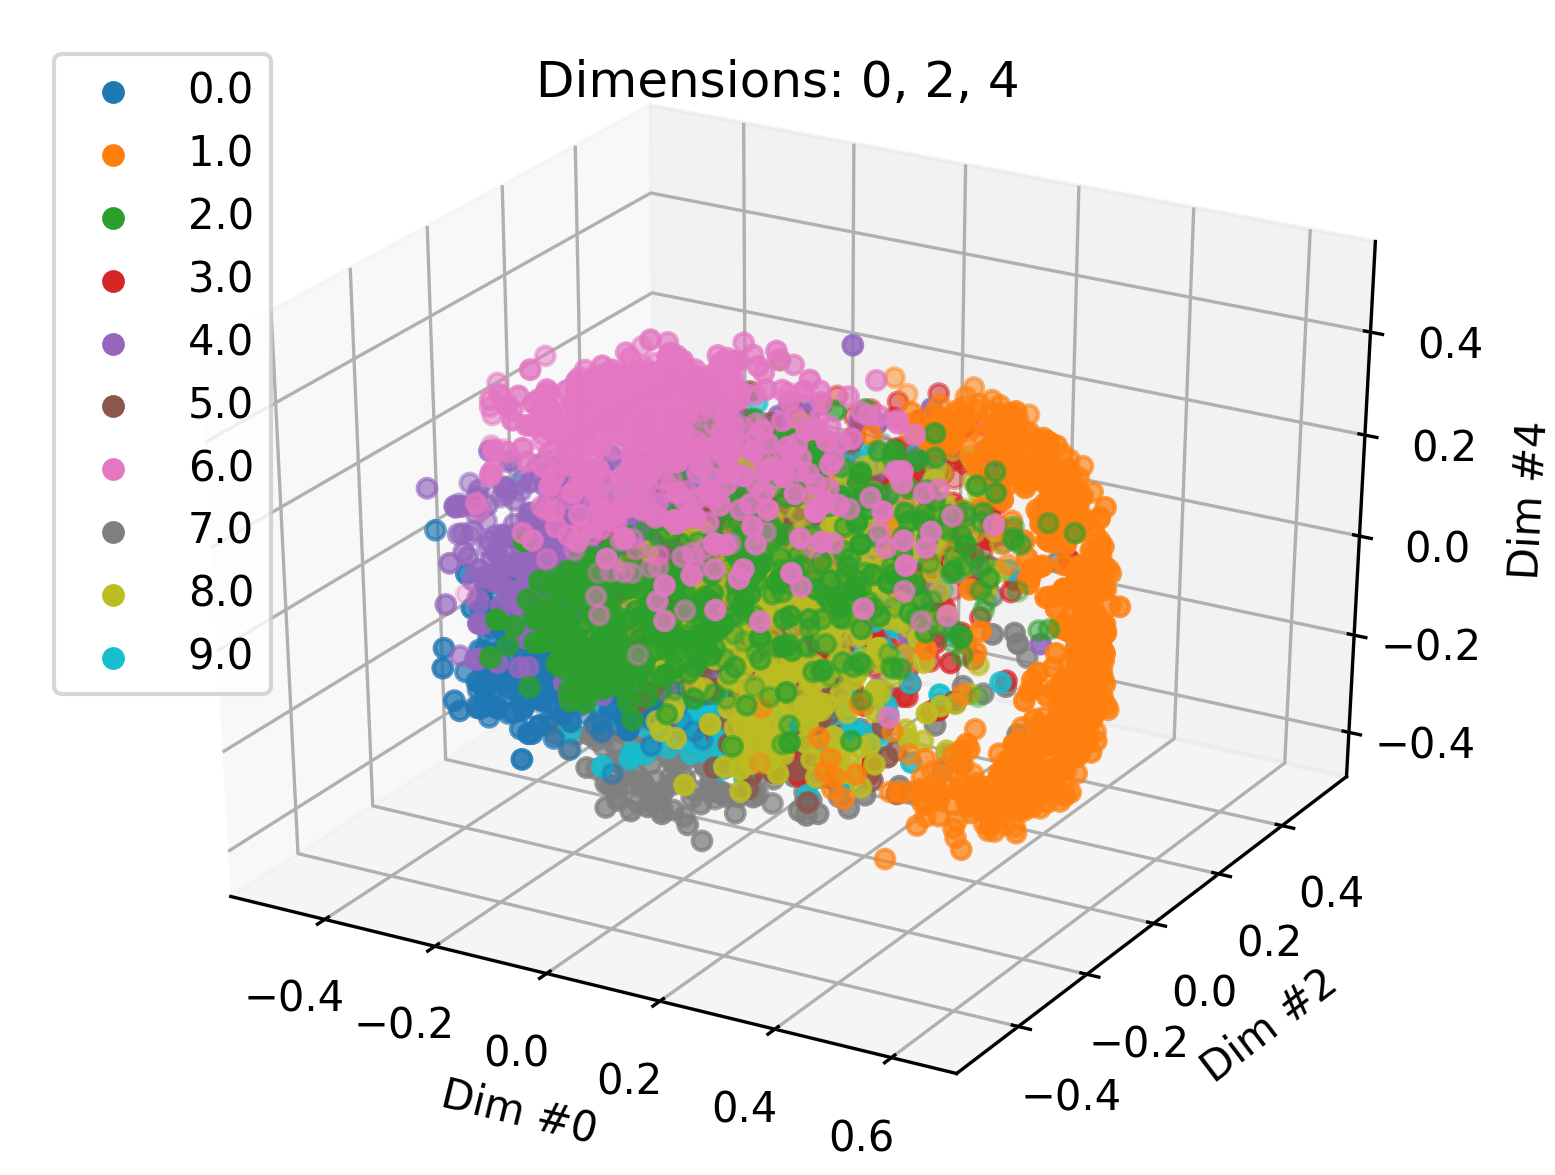
\includegraphics[width=0.23\textwidth]{pca/024.png}
  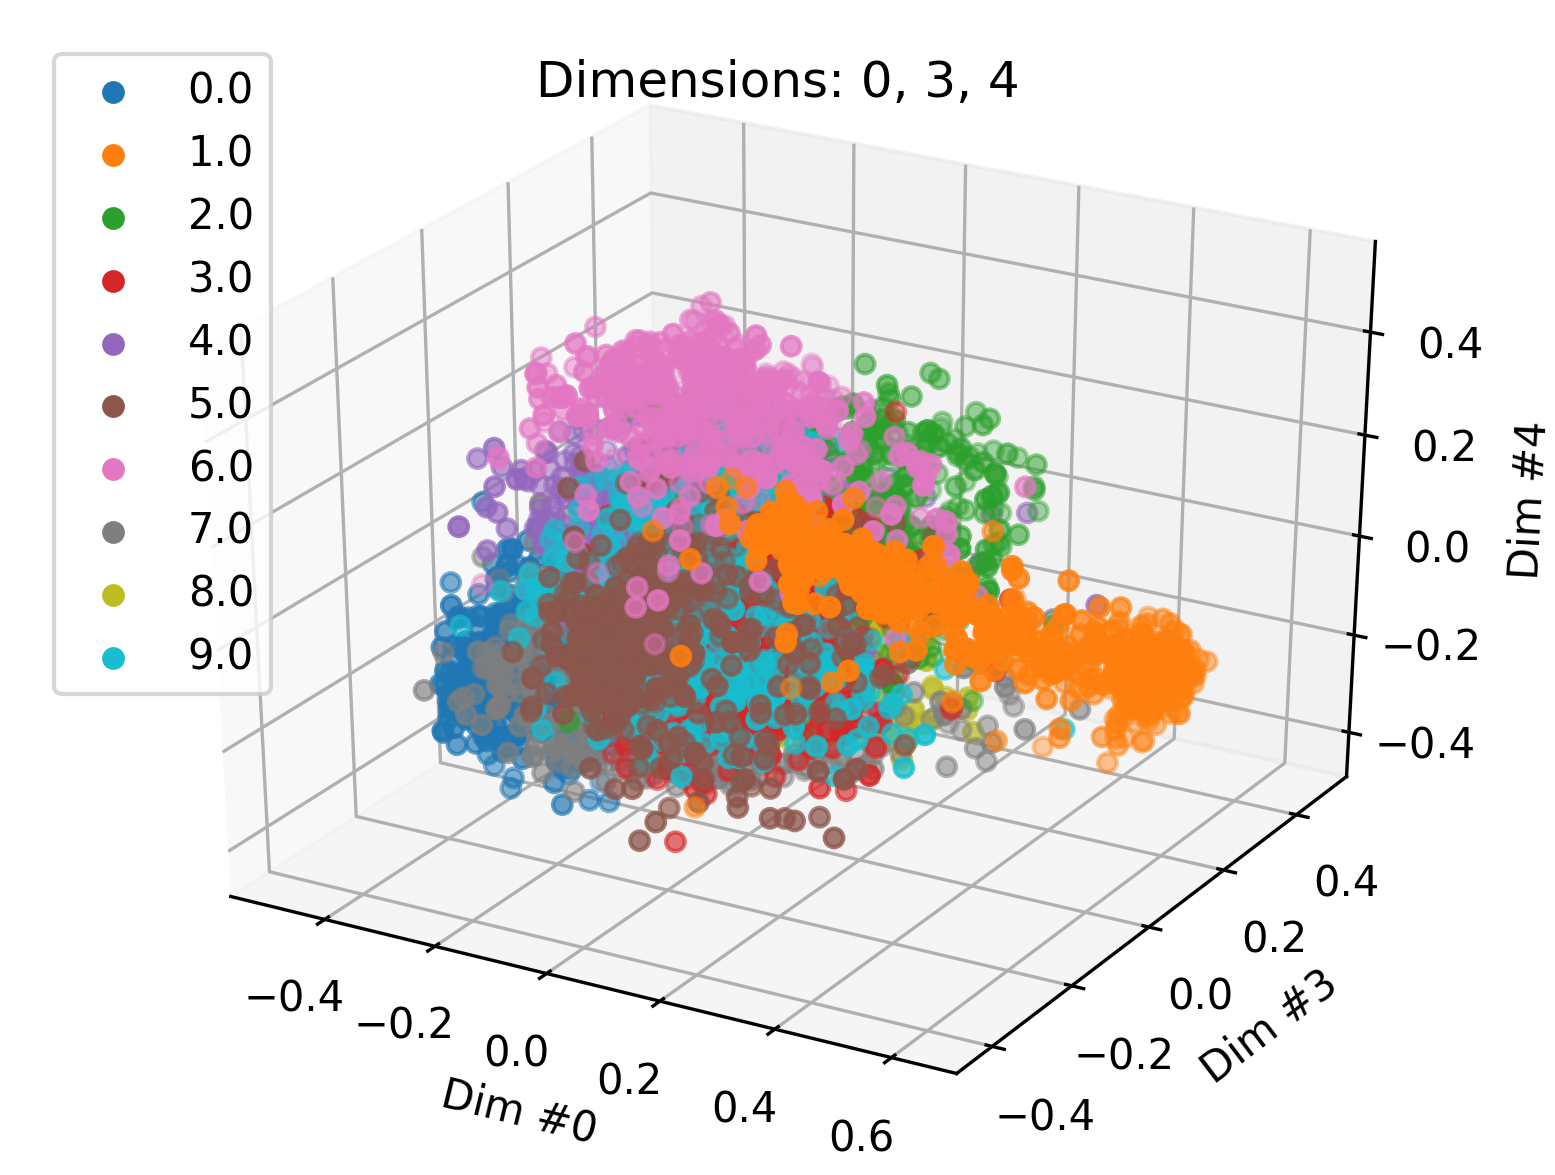
\includegraphics[width=0.23\textwidth]{pca/034.png}
  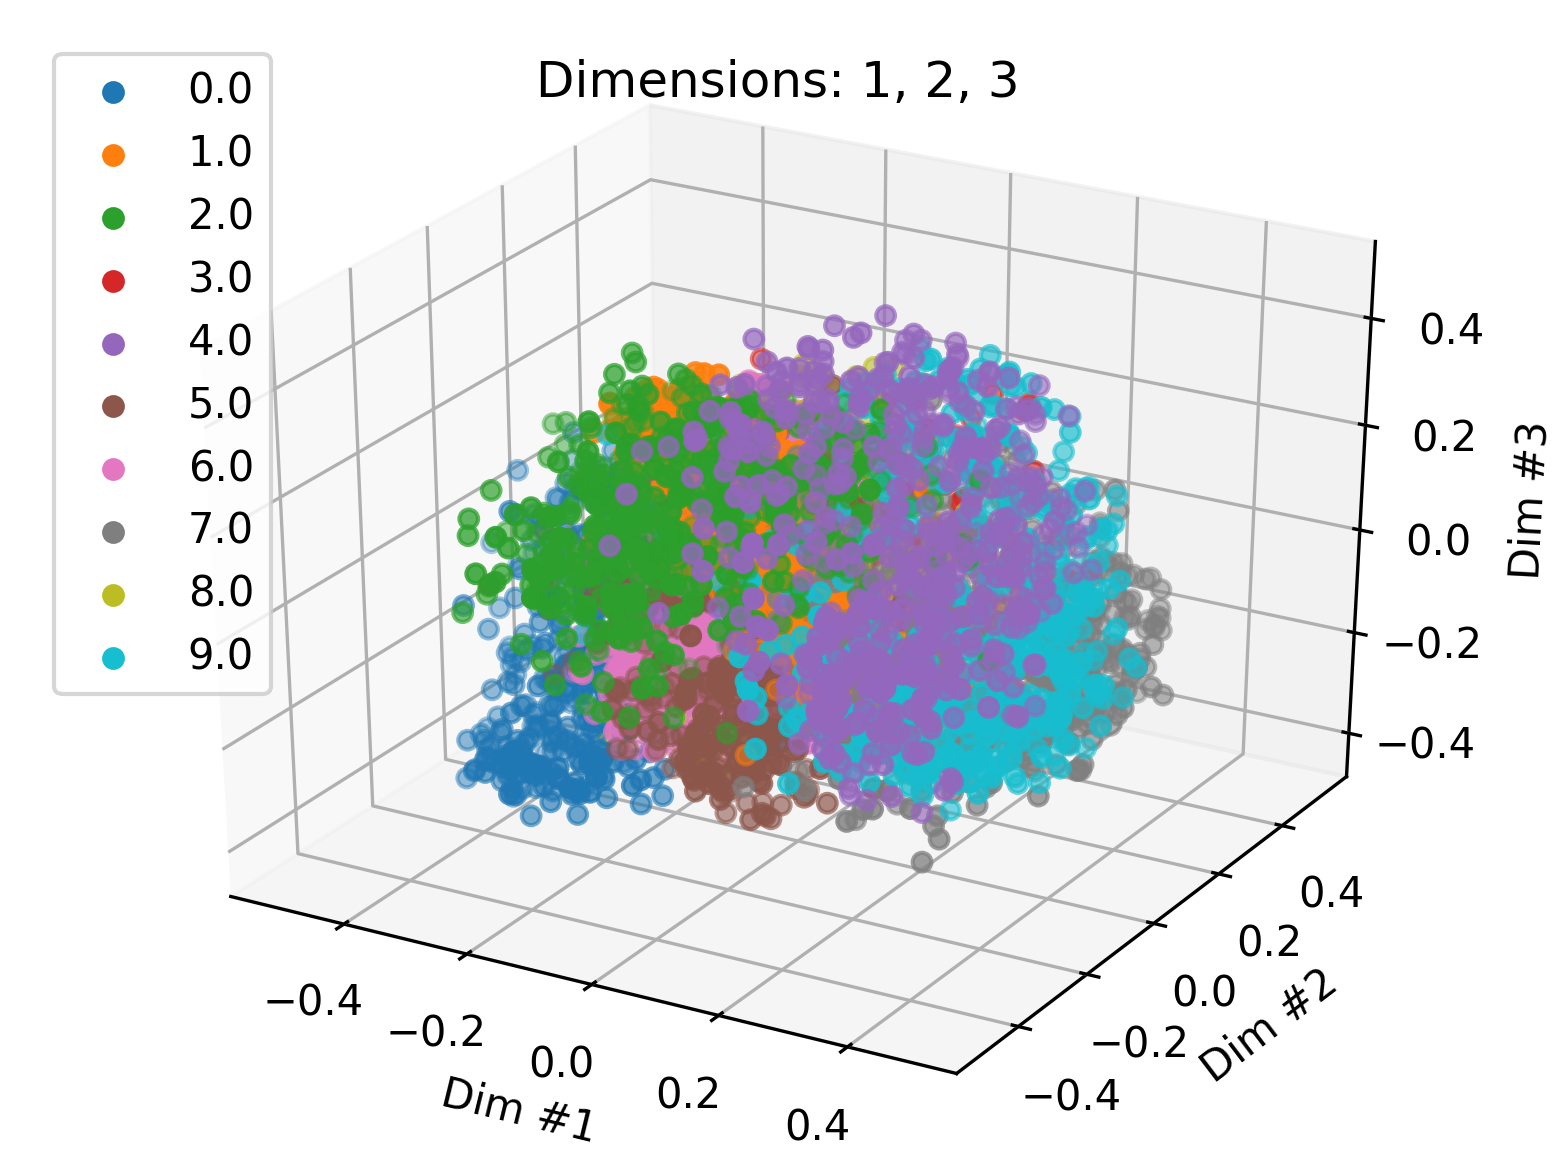
\includegraphics[width=0.23\textwidth]{pca/123.png}
  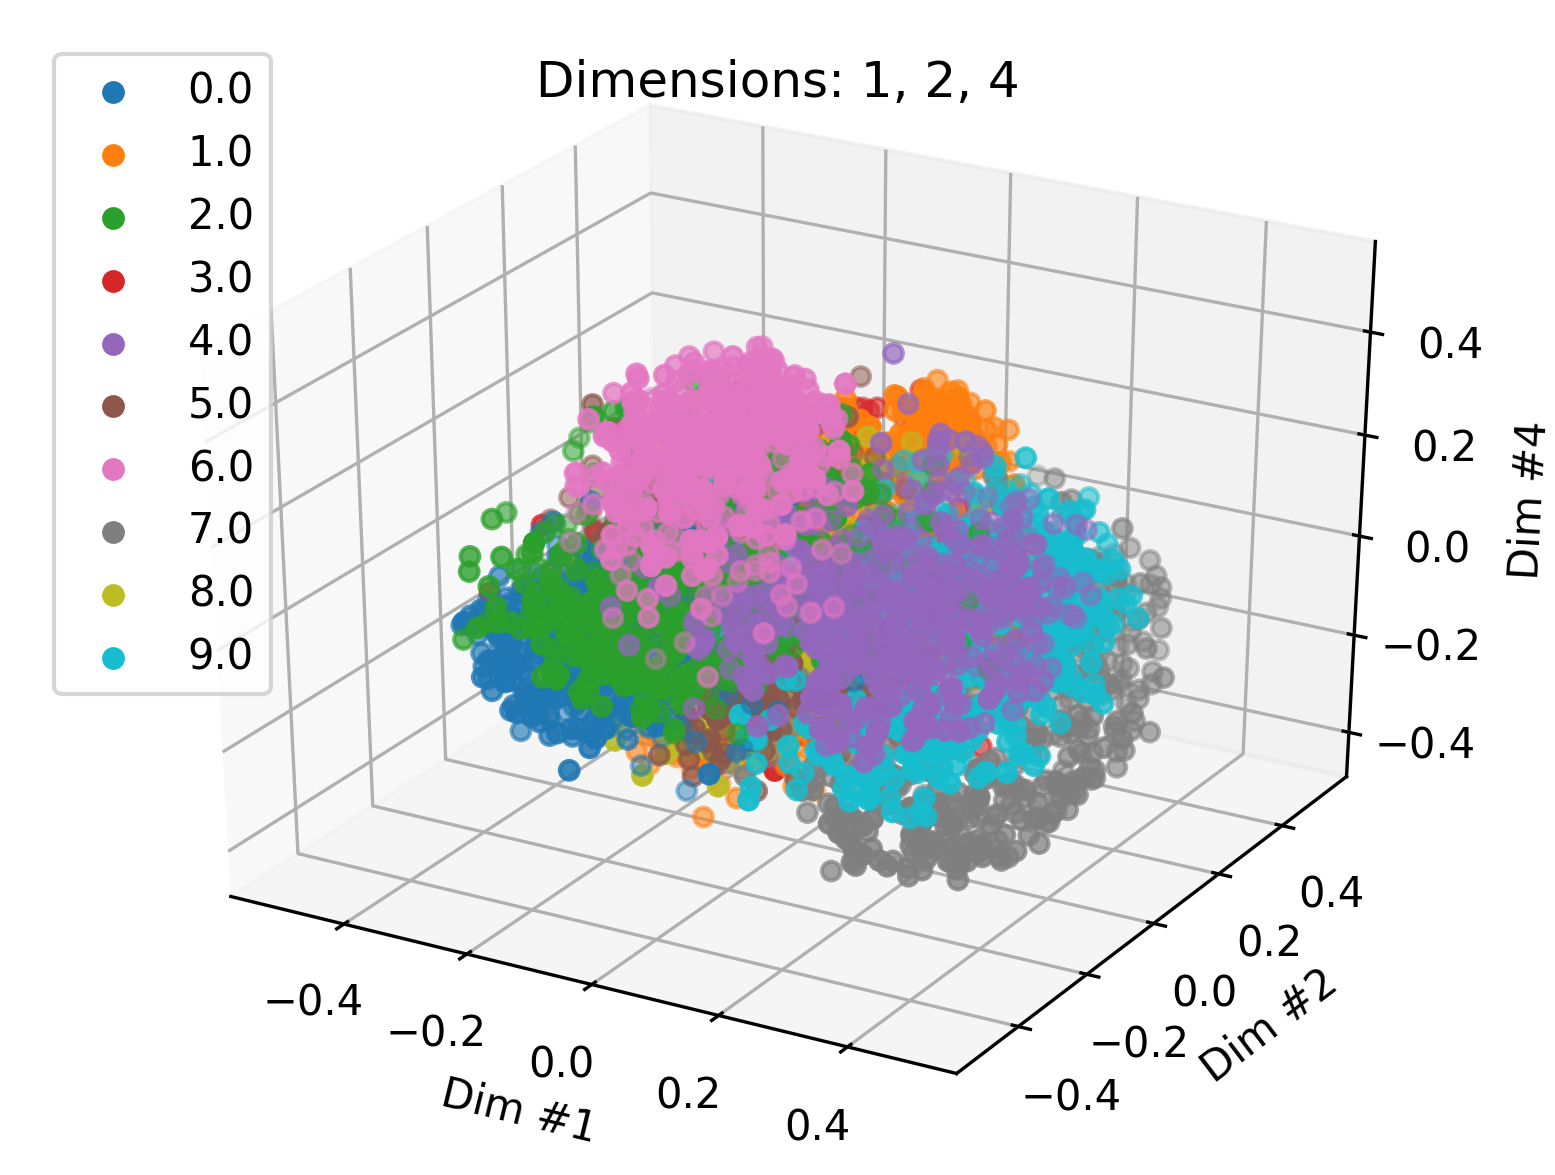
\includegraphics[width=0.23\textwidth]{pca/124.png}
  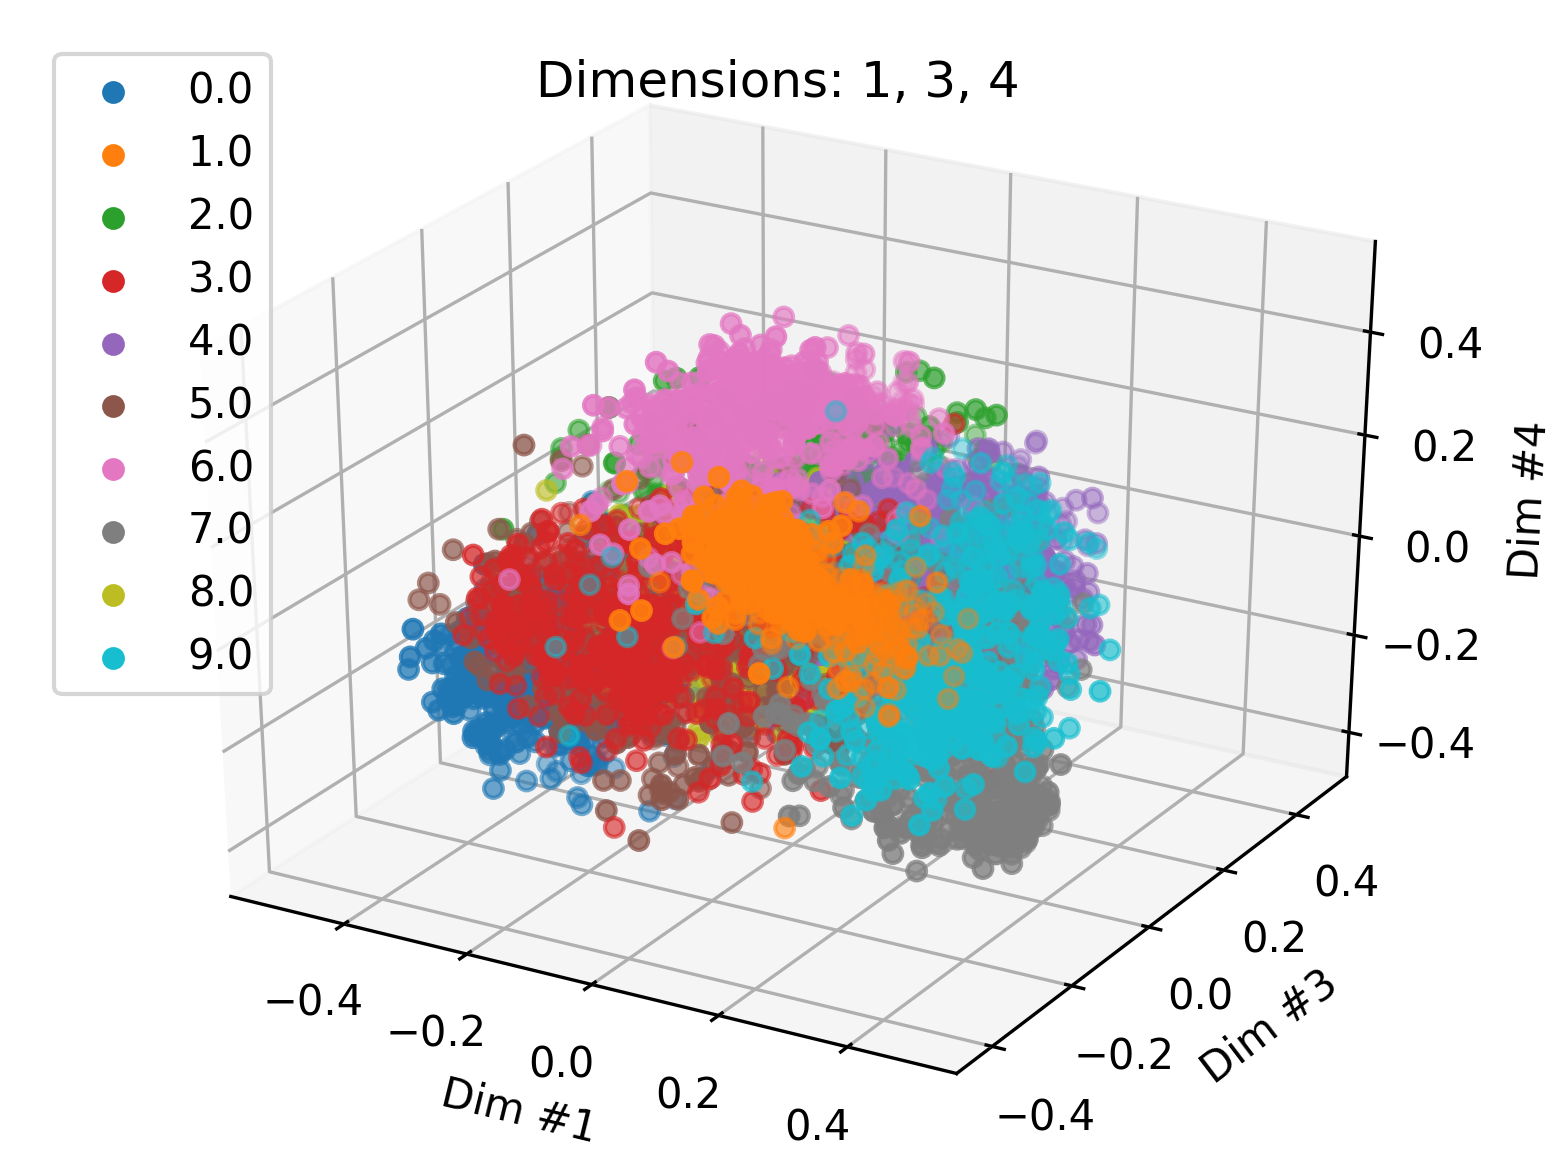
\includegraphics[width=0.23\textwidth]{pca/134.png}
  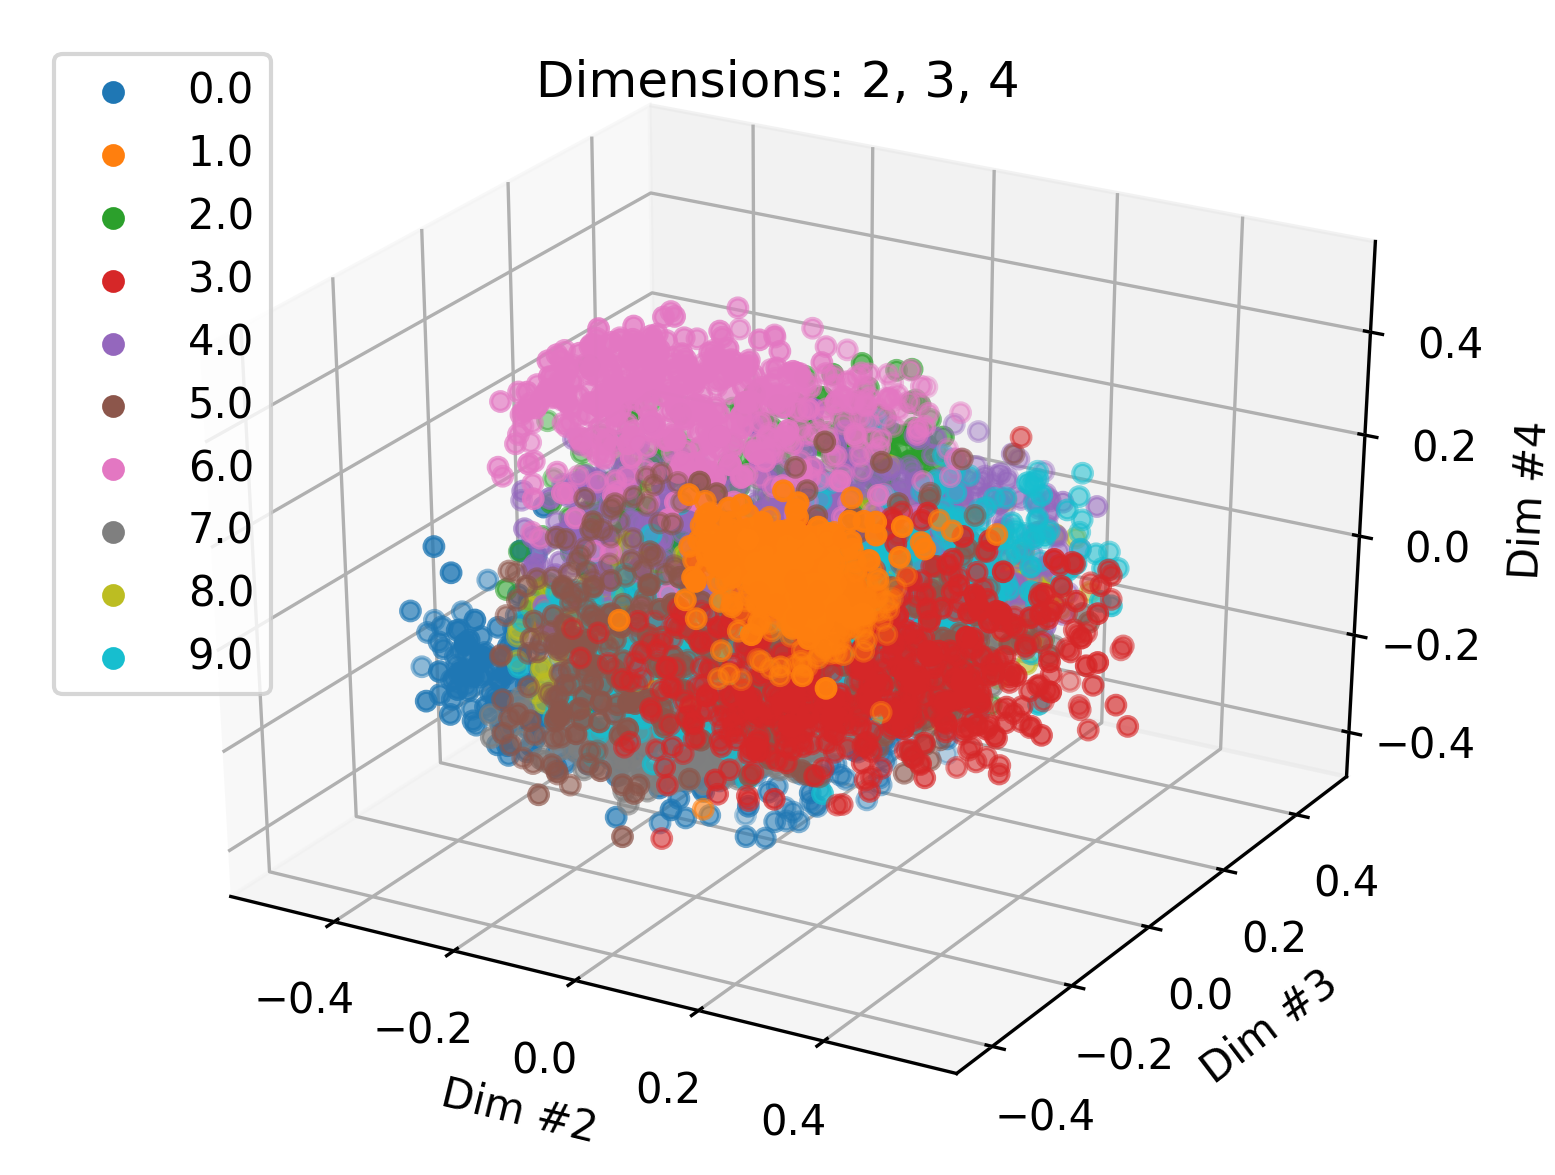
\includegraphics[width=0.23\textwidth]{pca/234.png}
  \caption{PCA graphs, coloured by the labels of the data.
           (Questions 2-6, part 1.)}
  \label{fig:pca_graphs}
\end{figure}

The `0'-labelled data points form distinct clusters in the figures containing
the zeroth dimension (i.e. the first principal component), but aside from this
it is difficult to identify distinct clusters in the data by eye.

To identify the most significant graph, we will use an informally-defined
measure of class separability --- i.e. in which graph the classes are the least
"mixed-up".  By eye, this seems to be either the graph with dimensions (0, 1,
3), as it has a very clearly distinct cluster for the `0'-labelled elements, or
the graph with dimensions (1, 2, 4), as it has fairly distinct class clusters.

For deeper analysis, an objective class separability measure could be used on
these 3-combinations of the principal components, but we will not do so
here.\footnote{This answers question 7 of part 1.}

\section{Competitive Learning} \subsection{Model and algorithm} The model used
for performing classification on the dataset was a single-layer artificial
neural network using a competitive learning mode, as outlined in \cite{hertz91}.
Briefly, for a normalised $n$-dimensional input vector and $m$ output units, we
randomly initialise $m{\times}n$ matrix $W$ of initial artificial synapse
weights.  Then, taking each input vector $\bm{\xi}^\mu$ in turn, we compute
$W\bm{\xi}^\mu$ to obtain an $m$-dimensional vector of postsynaptic inputs.  To
this, some noise is added and the postsynaptic neuron with the hightest input
firing rate is chosen to fire; all other postsynaptic neurons do not fire.  The
added noise serves the purpose of preventing so-called `dead units', which are
discussed further in \autoref{sec:deadunits}.

For the learning step, the weights of the synapses connected to the winning
postsynaptic neuron are adjusted in proportion to the difference between their
previous weight and the input vector.  The constant of this proportion, $\eta$,
is termed the \textit{learning rate}, and is one of the parameters used in
tuning.  In fact, as per the recommendation in \cite[p223]{hertz91}, we decided to use a
decaying learning rate of $\eta(t) = \eta_0t^{-\alpha}$ for some $0 \le \alpha
\le 1$, where $\alpha$ is known as the rate of decay of the learning rate.

Since this method does not require us to present all the training vectors before
calculating the weights, we can conclude that it is an \textbf{online} learning
algorithm --- that is to say, the algorithm could be paused after any step and
used for evaluation, and indeed more training data can be presented at any
stage.\footnote{This answers question 1 of part 2.  For further detail and code
snippets please see \autoref{sec:code}.}

It is necessary to $l_2$-normalise the input vectors before training in
order to correctly adjust the synaptic weights during learning.  If the input is
not normalised then the weights may grow infinitely --- so we must either apply
a normalising factor to the new weights after each training step, or simply
normalise our inputs before training \cite[p219]{hertz91}.

\subsection{Optimisation}

For the purposes of tuning, we use four parameters: the number of output units,
the learning rate, the weight of the added noise, and the rate of decay of the
learning rate.  From experimentation it seemed that the noise weighting did not
contribute significantly to any variations in accuracy of the network, so we
have held it constant at 0.005 for all presented evaluations.

For evaluating a trained network, we use the following procedure, using labelled
data:  Define $m$ artificial classes, one for each output unit, and classify
each input vector into one of these $m$ classes.  Then, assign a label (from
0--9) to each artificial class, based on which true class the majority of its
assigned inputs belong to.  (Thus, we obtain a mapping from our $m$ output units
to our 10 true class labels.)  Finally, count the number of correctly classified
inputs based on this mapping, and return this as a proportion of the total
number of inputs.  Using this method, a randomly initialised untrained network
will have an accuracy of \char"7E{}25\%.

In \autoref{fig:optimisation_graphs} are presented three 3-D graphs, showing the
accuracy as a function of two of the parameters under experiment, with an
average over the third.  These were obtained using the unreduced $28 \times 28$
data with 15 000 training iterations.  The values used for the learning rate,
learning rate decay, and number of outputs are $\eta = 1000^{-\frac{i}{10}}$,
$\alpha = 1000^{-\frac{j}{10}}$ and $m = k + 10$ respectively, where $i, j, k
\in \{0, \ldots, 10\}$.  These formulae for $\eta$ and $\alpha$ allow us to use
a high resolution near 0, where there is more variation and a lower resolution
further away.

What is clear from the graphs is that there is a maximum accuracy for some small
positive $\eta$ and $\alpha$.  In actual fact this maximum occurs at $(\eta =
0.032, \alpha = 0.002)$, which we later use in \autoref{sec:weight_change}.
Although there must exist a maximum on the $m$-axis, since for sufficiently
large $m$, our evaluation function will break down, finding it was beyond our
computational means.

\begin{figure}
  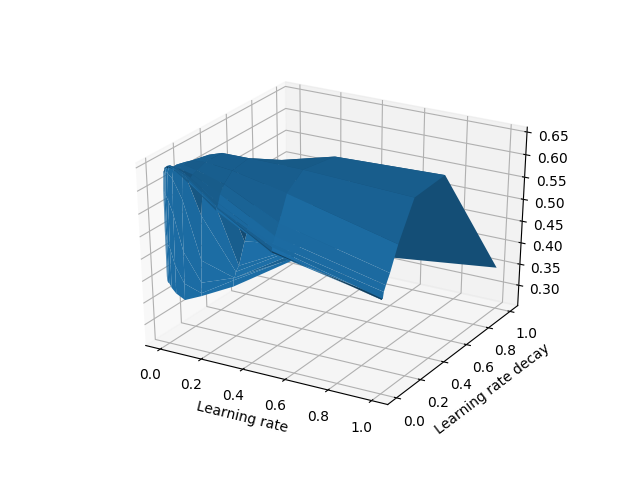
\includegraphics[width=0.46\textwidth]{optimisation/01.png}
  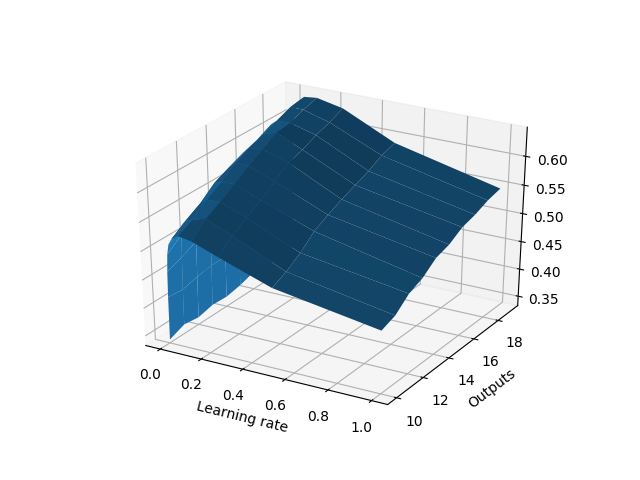
\includegraphics[width=0.46\textwidth]{optimisation/02.png}
  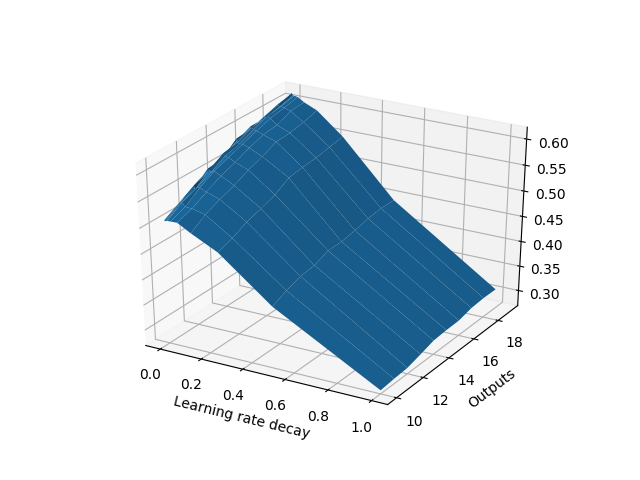
\includegraphics[width=0.46\textwidth]{optimisation/12.png}
  \caption{Performance curves for 3 parameters.}
  \label{fig:optimisation_graphs}
\end{figure}

\subsection{Dead units} \label{sec:deadunits} In the context of competitive
learning, a dead unit is defined as an output unit which enters a negative
equilibrium of never being activated for any input, and thus never learning. One
method of dealing with these units is to define some heuristic `dead unit
detection' function, and simply delete them.  In \cite[p221]{hertz91}, however,
some subtler approaches are outlined, for example using `leaky learning', in
which we update the weights of the losing units as well as the winning unit, but
with a small $\eta$, or smearing the output stimuli with noise, in order to give
a certain non-zero probability of firing to every output unit regardless of
stimulation.  The noise-smearing approach is what we implemented, and thus a
heuristic function for identifying dead units was never needed in our
case.\footnote{This answers question 4 of part 2.}

\subsection{Weight change} \label{sec:weight_change} A good measure of when a
network has learned sufficiently from the available data is to compute the
average synapse weight change over each training iteration.  When the training
reaches a constant, low-level rate of change, we can conclude that the network
is no longer learning anything useful.  \autoref{fig:weight_change} shows these
weight changes for a network with a learning rate of 0.032 and a learning rate
decay of 0.002 (the best result from the evaluation calculations above).  From
this we can see that after no more than \char"7E$2^{11}$ iterations, the
learning has stabilised and the network is about as good as it is ever going to
be with these parameters.\footnote{This answers question 5 of part 2.}

\begin{figure}
  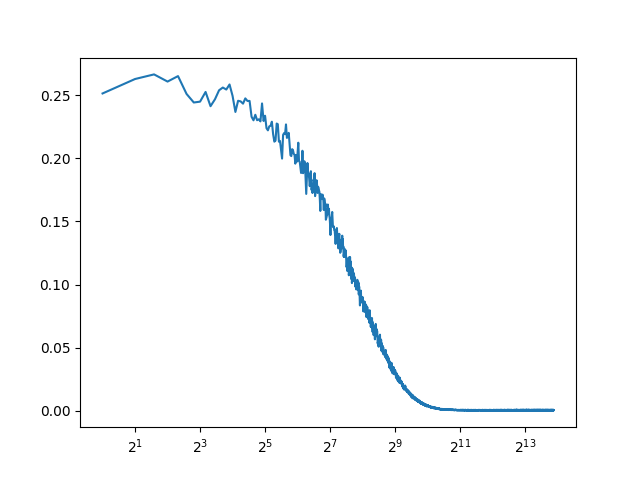
\includegraphics[width=0.46\textwidth]{dw_average.png}
  \caption{Moving average of $|\Delta{}\bm{w}_i|$ by iteration count.
           $\eta = 0.032$, $\alpha = 0.002$, $m = 15$, log-$x$ axis.}
  \label{fig:weight_change}
\end{figure}

\subsection{Final prototypes} On a network trained with $\eta = 0.032$, $\alpha =
0.002$, $m = 15$ for $2^{16}$ iterations, the final prototypes for each of the
$m$ output neurons are as displayed in \autoref{fig:weights}.  These are the
synapse weights for each postsynaptic neuron displayed in a $28\times28$ grid.
Clearly, it can be seen that each unit is specialised to recognise certain
common input patterns.\footnote{This answers question 6 of part 2.}

Additionally shown in the same figure is the $m\times{}m$ covariance matrix of
the prototypes. The bright diagonal line indicates the autocorrelation of each
prototype to itself, which is obviously high, and brighter squares outside the
diagonal indicate when two prototypes are similar.\footnote{This answers
question 7 of part 2.}

\begin{figure}
  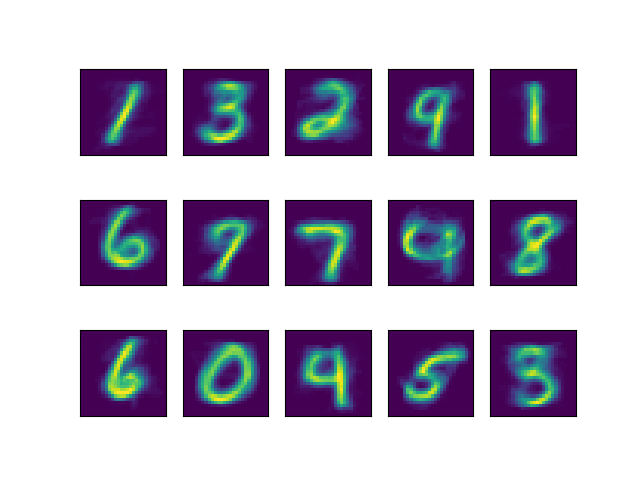
\includegraphics[width=0.46\textwidth]{weights.png}
  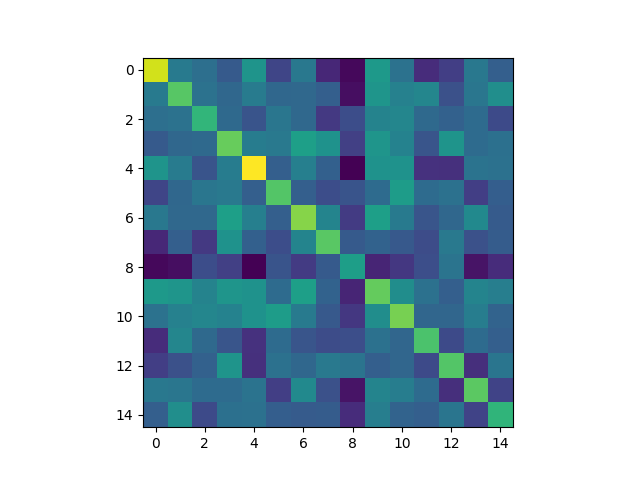
\includegraphics[width=0.46\textwidth]{unit_covariance.png}
  \caption{Final units and their covariance after $2^{16}$ iterations.
           $\eta = 0.032$, $\alpha = 0.002$, $m = 15$.}
  \label{fig:weights}
\end{figure}

\section{Reproducibility}
???

\begin{thebibliography}{9}
\bibitem{mnist}
  Y. Lecun and C. Cortes,
  ``The MNIST database of handwritten digits.''
  [Online].
  Available: \url{http://yann.lecun.com/exdb/mnist/}

\bibitem{numpy}
  Stéfan van der Walt, S. Chris Colbert and Gaël Varoquaux.
  ``The NumPy Array: A Structure for Efficient Numerical Computation'',
  Computing in Science \& Engineering, 13, 22--30 (2011),
  DOI:10.1109/MCSE.2011.37
  [Online].
  Available: \url{http://scitation.aip.org/content/aip/journal/cise/13/2/10.1109/MCSE.2011.37}

\bibitem{hertz91}
  J. Hertz \textit{et al.},
  ``Unsupervised Competitive Learning''
  in \textit{Introduction to the Theory of Neural Computation},
  Boulder CO: Westview Press,
  1991

\end{thebibliography}

\appendix \section{Code snippets} \label{sec:code} This appendix contains
listings of core parts of the codebase.  Auxiliary code, such as graph
generation, data classes, utility functions, etc. are omitted.

Throughout the code, we try to use a Pythonic style where possible, using NumPy
for fast work. Variable names are descriptive and it should be clear what the
algorithm is doing without too many comments.

\subsection{PCA} This code was re-used from a previous assignment in COM3004
(Data-Driven Computing).

\begin{lstlisting}[language=Python, style=python]
class PCAReducer(IdentityReducer):
    """Principle Component Analysis (PCA) dimensionality reducer.

    :param n: The number of dimensions (eigenvectors) to reduce to.
    """

    def __init__(self, n=40):
        """See class docstring."""
        self._n = n

    def train(self, train_data, *_, **__):
        """Train the PCA reducer.

        :param train_data: The training data to train on
        """
        cov = np.cov(train_data, rowvar=0)
        dim = cov.shape[0]
        _, eigenvectors = eigh(cov, eigvals=(dim - self._n, dim - 1))
        eigenvectors = np.fliplr(eigenvectors)
        self._eigenvectors = eigenvectors

        self._mean = np.mean(train_data, axis=0)
        getLogger('assignment.dimensionality.pca')\
            .info("Trained PCA reducer ({} -> {} dimensions)"
                  .format(dim, self._n))

    def reduce(self, data):
        """Reduce the provided data.

        :param data: The data to be reduced

        :return: The PCA-reduced feature vector(s)
        """
        centred_data = data - self._mean
        vs = self._eigenvectors[:, :self._n]
        getLogger('assignment.dimensionality.pca')\
            .debug("PCA-reduced some samples")
        return np.dot(centred_data, vs)

    def reconstruct(self, data):
        return np.dot(data, self._eigenvectors.T)
\end{lstlisting}

\subsection{Evaluations}
\begin{lstlisting}[language=Python, style=python]
class EvaluableClassifier(object):
    def evaluate(self, data, labels):
        classified = self.classify_many(data)

        # A confusion matrix is a table of true label vs. predicted label.
        confusion_matrix = np.zeros((self._inputs, self._outputs))
        for true_label, predicted_label in zip(labels, classified):
            confusion_matrix[int(true_label), int(predicted_label)] += 1

        # We evaluate each cluster's label by majority rule
        correspondence = np.argmax(confusion_matrix, axis=0)

        correct_results = 0
        for cluster_index, cluster_label in zip(
            range(self._outputs), correspondence):
            correct_results += confusion_matrix[cluster_label, cluster_index]

        return correct_results / np.sum(confusion_matrix)
\end{lstlisting}

\subsection{Neural network}
\begin{lstlisting}[language=Python, style=python]
class SingleLayerCompetitiveNetwork(EvaluableClassifier):
    def __init__(self, inputs, outputs, learning_rate=DEFAULT_LEARNING_RATE,
                 learning_rate_decay=DEFAULT_LEARNING_RATE_DECAY,
                 noise_weight=DEFAULT_NOISE_WEIGHT):
        self._inputs = inputs
        self._outputs = outputs
        self._learning_rate = learning_rate
        self._learning_rate_decay = learning_rate_decay
        self._noise_weight = noise_weight
        # Initialise the weights randomly for symmetry-breaking
        self._weights = np.random.rand(outputs, inputs)
        self._t = 0

    def train_one(self, data):
        self._t += 1

        output_firing_rate = np.dot(self._weights, data)
        noise = self._noise_weight * np.random.rand(self._outputs)

        # Add the noise to the firing rate and take the neuron with the largest
        # input
        winner_index = np.argmax(output_firing_rate + noise)

        eta = self._learning_rate * self._t ** (-self._learning_rate_decay)
        dw = eta * (data - self._weights[winner_index, :])

        self._weights[winner_index, :] += dw

        return winner_index, self._weights

    def train_many(self, data):
        return map(self.train_one, data)

    def classify_many(self, data):
        output_firing_rate = np.dot(self._weights, data.T)
        winners = np.argmax(output_firing_rate, axis=0)
        return winners
\end{lstlisting}

\end{document}
% Disable intented paragraphs and add space between them instead.
% \setlength{\parskip}{10pt}
% \setlength{\parindent}{0pt
